% !TEX root = ../main.tex
\documentclass[../main.tex]{subfiles}
\begin{document}
\label{sec:method}

\subsection{The Galaxy Builder Zooniverse project}

Galaxy Builder is a citizen-science project built on the Zooniverse\footnote{\url{https://www.zooniverse.org}} web platform. It asks volunteers to perform detailed photometric modelling of spiral galaxies (including the bulge, disk, bar and spiral arm components). As a project of this kind, allowing users to interact with and model data, had never been attempted inside the Zooniverse web platform before, we had to design and implement a (comparatively basic) model rendering suite inside the existing Zooniverse front-end code-base. We had to not only consider the accuracy of the resulting model, but also user experience and engagement in our design decisions.

The closest relative to this project within the Galaxy Zoo ecosystem was the Galaxy Zoo: Mergers project \citep{Holincheck2016:1604.00435v1}. This project asked volunteers to help match the morphological properties of an image of merging galaxies to a plethora of restricted three-body simulations, in an attempt to identify the possible initial conditions resulting in the observed morphology. For part of the project, volunteers downloaded a Java applet, which would run restricted three-body simulations and generate output images. The volunteer then voted on simulations which matched a given galaxy merger image, or shared important tidal features. A new batch of simulations would then be run.

\subsubsection{Project Timeline and Development}

The Galaxy Builder project was developed over one and a half-years, and was built inside the Zooniverse's \textsc{Panoptes-Front-End}\footnote{\url{http://github.com/zooniverse/Panoptes-Front-End}} codebase, using Facebook's \textsc{React.js}\footnote{\url{https://reactjs.org/}} framework, as well as WebGL\footnote{\url{https://www.khronos.org/webgl/}} to enable realtime photometric galaxy model rendering. Galaxy Builder entered a Zooniverse beta in late November 2017 and after some user experience improvements and significant code reworking to meet internal standards, the project was launched as an official Zooniverse project on the 24th of April 2018.

A major challenge during development of the project was finding the right balance between keeping the interface and instructions simple enough for users to understand intuitively, while also allowing the freedom and versatility to properly model galaxies. It was also a significant challenge to develop a compelling and simple tutorial for what is one of the most complex projects attempted on the Zooniverse platform.

\subsubsection{The project interface}

The Galaxy Builder project presents a volunteer with three images, which they can switch between at any time: an $r$-band cutout of a spiral galaxy (for details of the images used see Section \ref{sec:data}), the galaxy model they have created so far, and the residual between their model and image (shown in blue and yellow). A screenshot of the interface can be seen in in Fig.\ref{fig:interfaceInProgress}.

\begin{figure*}
  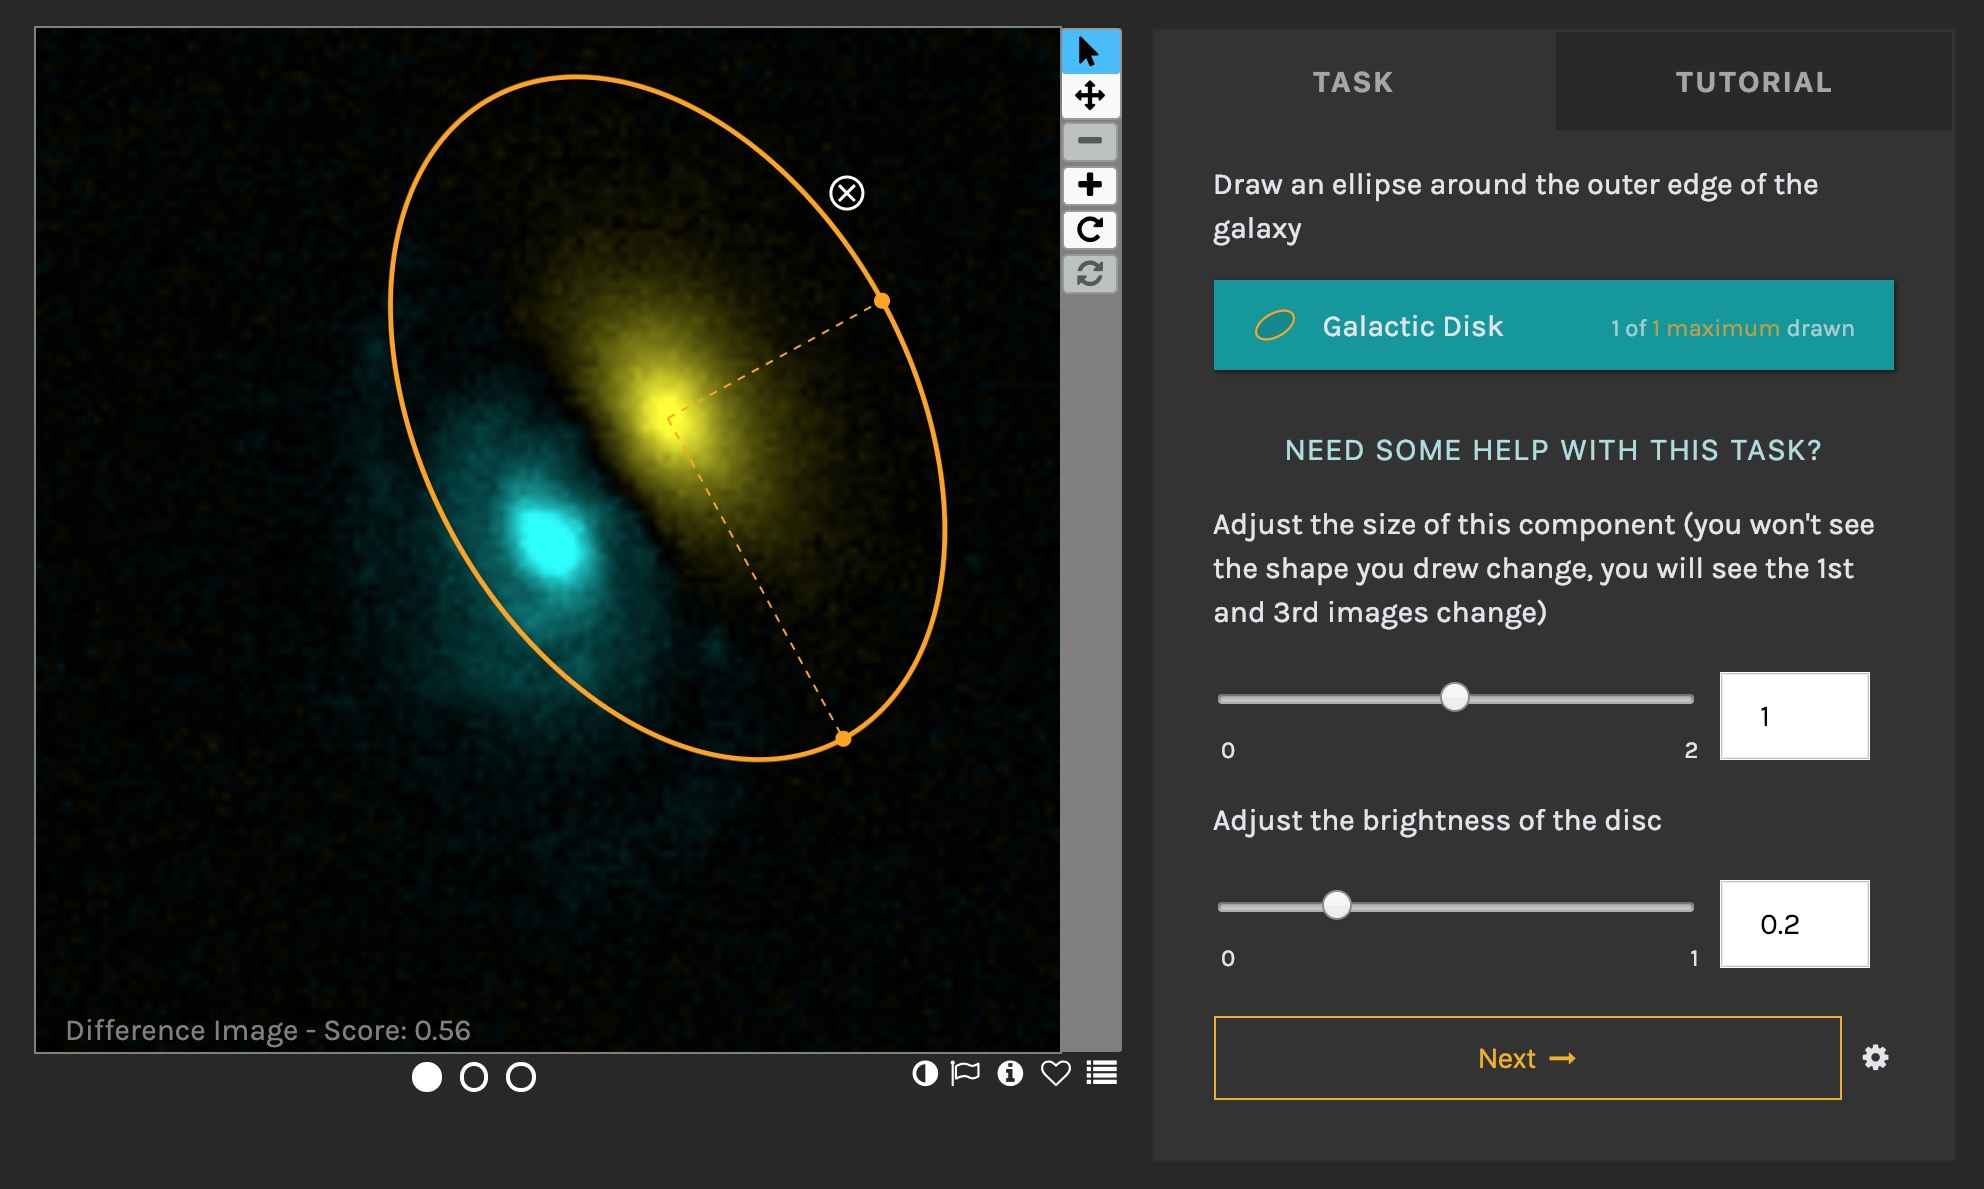
\includegraphics[width=17.7cm]{images/interfaceInProgress.jpg}
  \caption{The galaxy builder interface. The residual image is being shown, and the volunteer is on the ``Disc'' task. The drawn disk component (yellow) is offset from the galaxy image (blue) to demonstrate the positive and negative residuals. Where the image equals the model the residual is black.}
  \label{fig:interfaceInProgress}
\end{figure*}

The interface prompts volunteers to work through the step-by-step creation of a photometric model of a galaxy (described in detail in Section \ref{section:galaxy-model}). At each step volunteers are asked to first draw a simple isophote (ellipse for disk and bulge, rectangle for bar and polygon-lines for spiral arms), and then make use of a series of sliders to adjust the parameters of the model component (i.e. brightness, S\'ersic index and boxyness).

The workflow is designed so that volunteers slowly subtract increasing amounts of light from the galaxy, as can be seen in Fig.\ref{fig:residualsStepByStep}. A tutorial is present which contains a step-by-step guide to completing a classification.

Volunteers are also guided by a ``score'', which is tied to the residuals and chosen to increase from zero to some unknown value depending on the galaxy provided; a less noisy and more easily modelled galaxy will be capable of a higher maximum score. To map a residual image to a final score shown to volunteers we used

\begin{equation*}
    S = 100 \exp\left(\frac{-A}{N}\sum_{i=0}^N\frac{\text{arcsinh}^2\left(\,|\text{y}_i - M_i|\ /\ 0.6\right)}{\text{arcsinh}\,0.6 }\right)
\end{equation*}

where $N$ is the total number of pixels, $y$ is the cutout of the galaxy, normalized to a maximum value of 1 ($y = \text{cutout}/\text{max}(\text{cutout})$), $M$ is the model calculated by volunteers and $A=300$ is an arbitrary choice of scaling chosen based on a handful of test galaxies.

This score has the advantage of being easy (and fast) to calculate from the residual image shown to voluteers (which was Arcsinh-scaled in a manner described by \citealt{Lupton2003:astro-ph/0312483v1}), however it is overly sensitive to small deviations of the model from the galaxy. Based on experience running the project, we don't think results are highly sensitive to what ``score'' was shown but would recommend a simpler error measure to future similar projects.

\begin{figure}
  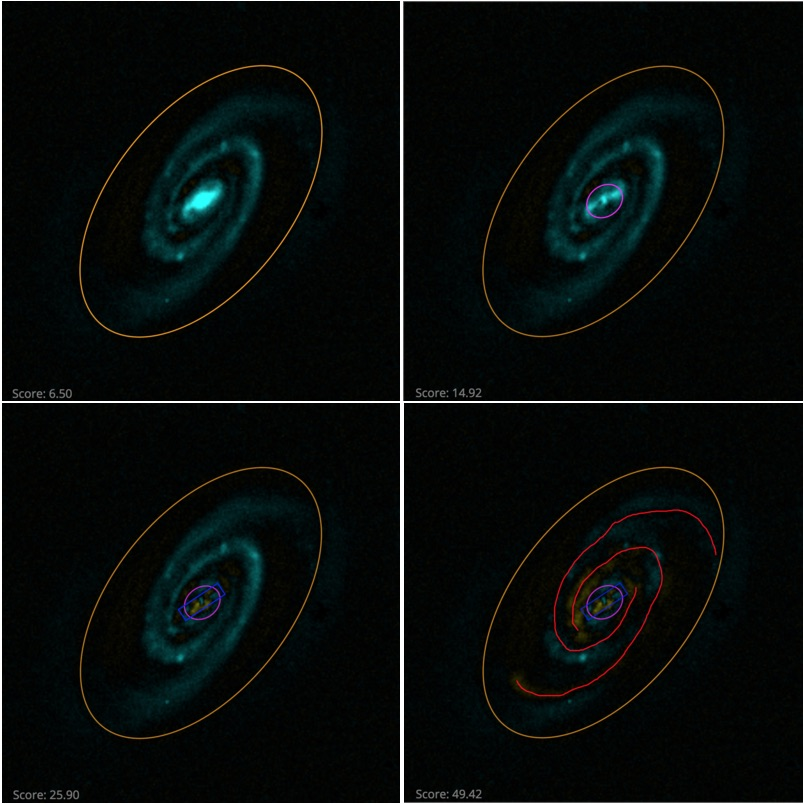
\includegraphics[width=8cm]{images/residualProgress.jpg}
  \caption{Figure demonstrating the ideal result of each step of the classification process. The top left panel shows the galaxy after only a disk component has been added: the top right contains a disk and a bulge; the bottom left has a disk, bulge and bar; the bottom right is the finished model with a disk, bulge, bar and spiral arms. The galaxy shown is SDSS J104238.12+235706.8. This brightness and contrast of this image have been edited to improve visibility in print.}
  \label{fig:residualsStepByStep}
\end{figure}

\subsubsection{Rendering the model}

We use the term rendering in a similar manner to that used for computer graphics: to calculate an image from a model or set of rules.

The rendering code used in the Galaxy Builder project was designed to run on a computer's GPU, using the WebGL rendering API (via the high-level Javascript interface \textsc{regl}\footnote{\url{http://regl.party/}}). This enables the model (and residual) to be calculated at a speed which allows low-latency feedback to a change in the model made by the volunteer in the browser. We do experience problems with some computers and browsers not being able to render models, which we detect and prompt volunteers to use a compatible browser. Our choice also has the impact of limiting precision of the model to that allowed by WebGL. As these models are envisioned as a starting point for a later numerical fit, it was determined this precision was sufficient.

\subsection{Images and Ancillary Data}
\label{sec:data}
The original sample proposed for the Galaxy Builder project aimed to mirror the \textit{stellar mass-complete sample} in \citet{Hart2017:1708.04628v1}. This was a sample of face-on spiral galaxies, with and without bars, complete in stellar mass. The morphological information required to select spiral galaxies came from the public data release of Galaxy Zoo 2 (\citealt{Willett2013:1308.3496v2}, hereafter GZ2). Each response to a GZ2 morphology question is allocated a $p$ value ranging from 0 to 1, where 0 indicates no volunteers responed positively to that question and 1 indicates all volunteers who classified that galaxy responded positively (i.e. $p_\text{bar} = 0.5$ would indicate $50\%$ of volunteers said a bar was present in a galaxy). Photometric measurements used for selection came from the NASA-Sloan Atlas \citep{2011AJ....142...31B}. The \textit{stellar mass complete sample} is constructed using the following:

\begin{itemize}
  \item GZ2 $p_\text{features} \cdot p_\text{not edge on} \cdot p_\text{spiral} \ge 0.5$
  \item $0.02 < z < 0.055$
  \item g-band axial ratio $a/b > 0.4$
  \item r-band magnitude $14 < m_r < 17$
  \item Computation of stellar mass completeness limits using the method of \citet{Pozzetti2009:0907.5416v2} and limits calculated by \citet{Hart2017:1708.04628v1}
  \begin{itemize}
    \item Exclusion of galaxies outside these limits\\
      $\log({M_* / M_\odot}) > 2.07\log(z) + 12.64$\\
      $\log({M_* / M_\odot}) < 2.45\log(z) + 14.05$.
  \end{itemize}
  \item A volume correction, excluding galaxies outside $9.45 < \log(M_* / M_\odot) \le 11.05$
\end{itemize}

This selection criteria results in the \textit{stellar mass-complete sample} of 6222 spiral galaxies. We do not obtain volunteer classifications for all of these, but a sub-selection of 198 (the selection of these is detailed in section \ref{sec:retirement-limit}).

\subsubsection{Image and modelling metadata extraction}

The galaxy data shown to volunteers in the Galaxy Builder project came in two forms: A gray-scale image cutout of the galaxy and a JSON file containing rendering information for the web-interface.

Both forms of data were obtained using a similar process:

\begin{itemize}
\item A montage of multiple r-band observations from the SDSS DR13 data release was created. To combine multiple FITS images, we made use of the \textsc{Montage}\footnote{Montage is funded by the National Science Foundation under Grant Number ACI-1440620, and was previously funded by the National Aeronautics and Space Administration's Earth Science Technology Office, Computation Technologies Project, under Cooperative Agreement Number NCC5-626 between NASA and the California Institute of Technology.} software package.\footnote{Two out of the two-hundred selected galaxies failed to run through the image preparation process, due to an error when attempting to montage multiple frames. The root cause of this error is unknown.}
\item This montage was cropped to four times the Petrosian radius of the galaxy.
\item The \textsc{SExtractor} software \citep{source-extractor} was used to identify regions containing foreground stars and generate a mask.
\item The JSON file was written containing the cut-out data and the 2D boolean mask obtained from the source extraction process. This file also contained other metadata needed for the rendering process (PSF, the size of the PSF array, and the width and height of the image).
\item Another JSON file containing simply the information used to render the volunteer's model (image size and PSF) was created.
\item An asinh-stretch was applied to the masked cutout (as described by \citealt{Lupton2003:astro-ph/0312483v1}). It was then saved as a grey-scale image.
\end{itemize}

We chose to use r-band images in our subject set due to it's higher signal-to-noise than other bands.

Once a sub-sample had been created, the Zooniverse's \textsc{panoptes-python-client}\footnote{\url{https://github.com/zooniverse/aggregation-for-caesar}} \citep{coleman_krawczyk_2019_2562861} was used to upload them as a subject-set to the Zooniverse.


\subsection{The Galaxy Model}
\label{section:galaxy-model}

The model we chose was largely based off of components and methodology described in \citet{galfit-paper}. The chosen model components were: An exponential, elliptical disk; an elliptical S\'ersic bulge; a S\'ersic bar with a ``boxiness'' modifier on the isophote; spiral arms drawn using freehand lines.

Each spiral arm is modelled using a polygon-line drawn by the volunteer. The brightness of a spiral arm at any point is given by the value of a Gaussian centred at the nearest point on any drawn polygon-line, with users able to choose the Gaussian spread and peak brightness using sliders. Radial falloff was added by multiplying by the value of the previously added exponential disk, though volunteers could change the half-light radius of this falloff disk.

The decision to render spirals in this manner was chosen to accommodate irregular spiral patterns drawn on by volunteers in a simple but acceptably realistic manner. It was decided that the actual spiral profiles were less important to the reduction and analysis process than the positions of the drawn polygon-lines.

The modelling code correctly ignores masked regions identified in the images. It over-samples the bulge, disk and bar components to a factor of five and performs PSF convolution using a PSF obtained in the subject set creation process.

\subsection{Choice of Retirement limit}
\label{sec:retirement-limit}

As we were unsure as to the rate at which volunteers would be able to classify images, we split the \textit{stellar mass-complete sample} into smaller sub-samples, each containing 100 galaxies. In an iterative process we chose each sub-sample to contain 60 of the lowest redshift galaxies and 40 random galaxies of those remaining in the sample.

After collecting data for two of these sub-samples, preliminary analysis of the classifications indicated that, in order to be able to reliably calculate an aggregate model, we needed more classifications per galaxy than the 10 we had originally envisioned.

A hand-picked sample of 56 galaxies was then re-activated with a retirement limit of 30 classifications per galaxy. This sample was chosen by eye to be a relatively diverse set of galaxies, most with prominent spiral features including grand-design and flocculent arms. Its purpose was to allow preliminary aggregation methodology development.

Once this hand-picked sample was completed, the remaining galaxies from the initial two sub-samples were re-activated, as well as a repeat of the first sub-sample (hereafter the \textit{validation subset}) to measure volunteer consistency. At the time of writing, only these three batches of galaxies have been run through the project.


\subsection{Classification Aggregation Methodology}

We will use galaxy UGC 4721 as an example galaxy for the illustration of the data reduction and aggregation methodology. For UGC 4721 we received 32 classifications, containing 28 disks, 24 bulges, 17 bars and 47 drawn spiral arm poly-lines. These annotations can be seen in Figures \ref{fig:drawn_shapes} and \ref{fig:drawn_polylines} \comment{merge these figures}.

\subsubsection{Disk, Bulge and Bar Aggregation}

\begin{figure*}
  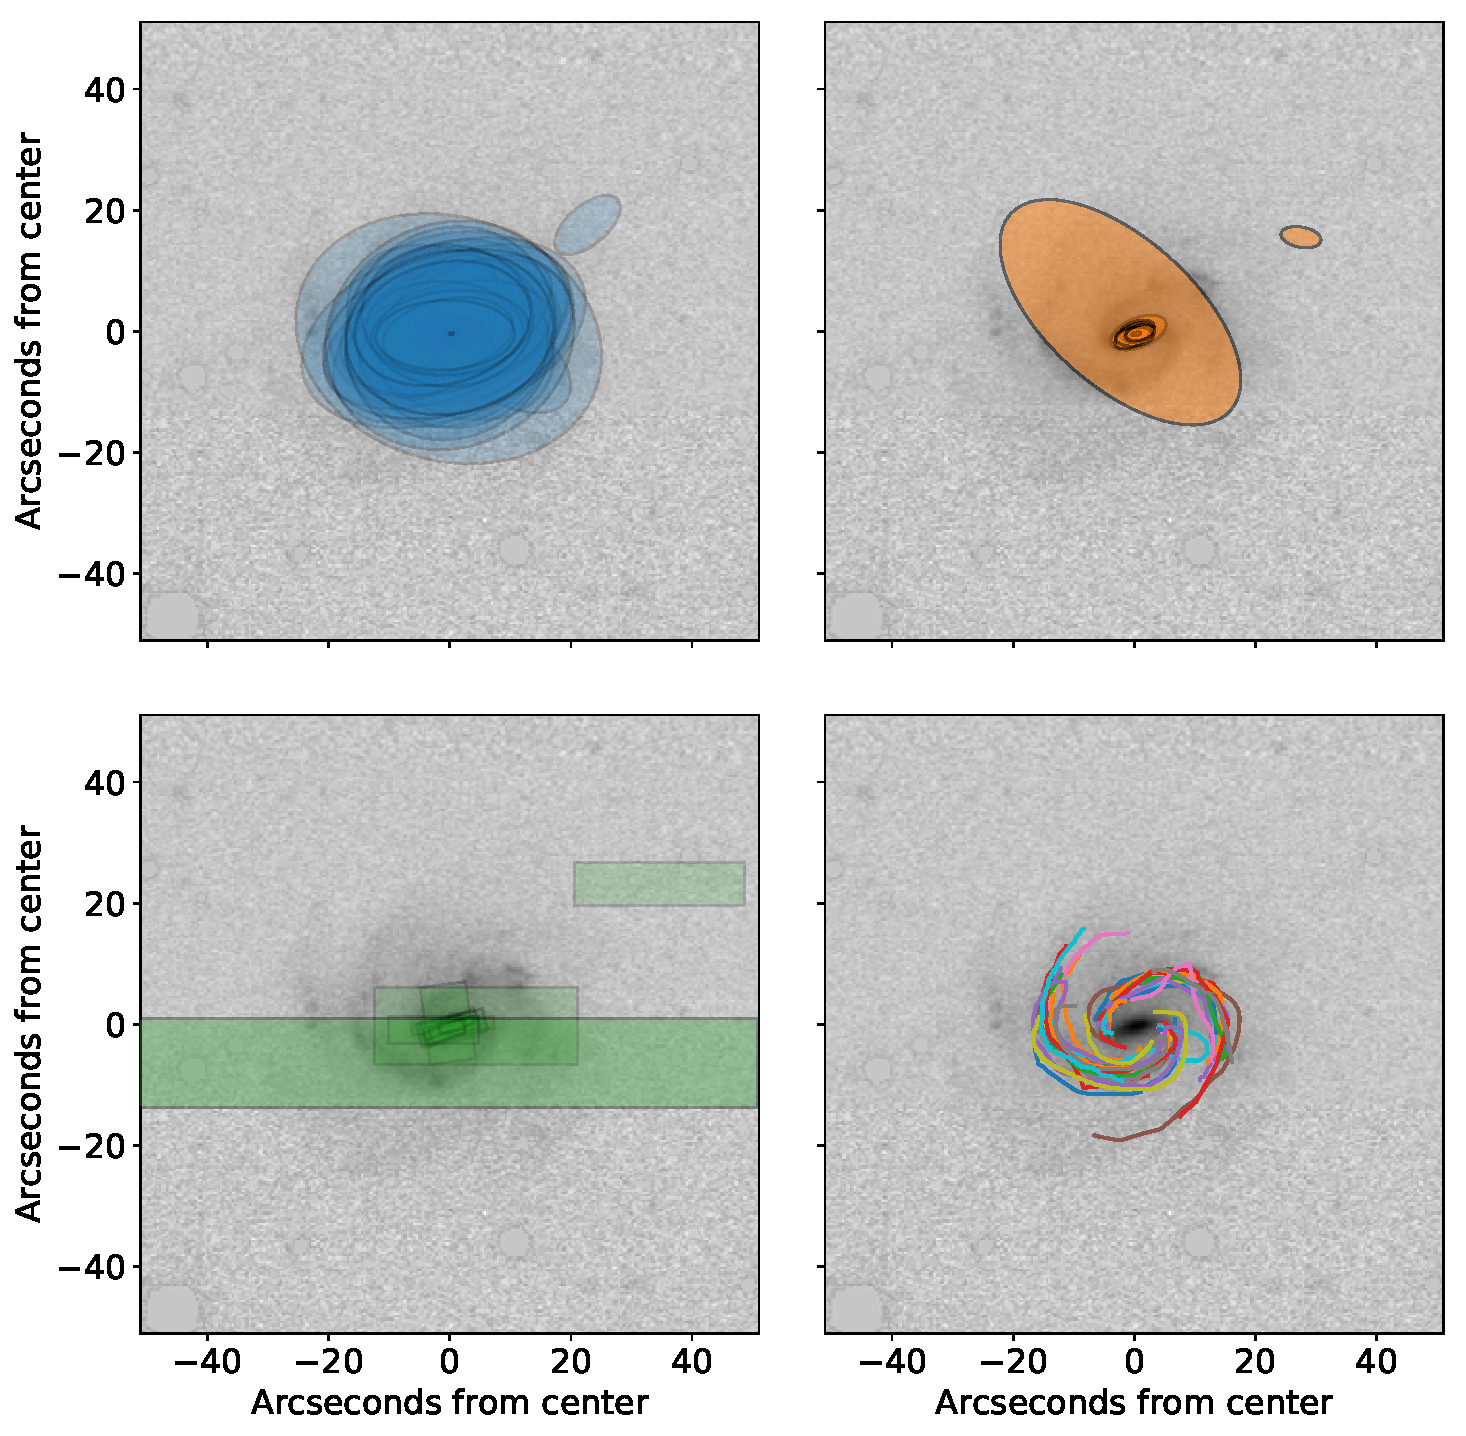
\includegraphics[width=15cm]{images__results/drawn_shapes.pdf}
  \caption{Example of drawn components for UGC 4721}
  \label{fig:drawn_shapes}
\end{figure*}

Clustering the disk, bulge and bar components was done purely on the shapes drawn by volunteers, as preliminary data exploration suggested that some users simply left model parameters at their default values, or moved them to an extreme of the allowed range. These shapes can be used as the starting point for numerical fits.

Clustering was done using the Jaccard distance measure, which is a simple metric determining the relative shared area of two shapes:

\begin{equation}
d_J(A, B) = 1 - \frac{|A \cap B|}{|A \cup B|}.
\end{equation}

The algorithm chosen to perform clustering was the Density-based spatial clustering of applications with noise (DBSCAN, \citealt{dbscan}) algorithm, due to its robustness and speed. We made use of Scikit-learn \cite{scikit-learn} to implement the algorithm. The parameters \texttt{eps} and \texttt{min\_points} were chosen by visually inspecting the resulting clustering results.

For shapes clustered in this way, we define their mean to be the shape which minimises the sum of Jaccard distances to each of the shapes in the cluster.

% An alternate method explored to calculate the mean shape of a cluster was to calculae the means of the parameters (width / height / position / roll) of the shapes in the cluster. Mean rotation was calculated using the \texttt{avg\_angle} function inside the Zooniverse's \textsc{panoptes-aggregation} package. This properly minimises the mean squared error (which many formulas do not), whilst also respecting isophotal symmetries.
%
% I.e. the angle $\bar{\phi}$ which minimises
%
% \begin{equation}
%     D = \sum_{i=0}^n \left(\phi_i \bmod \phi_\text{max} - \bar{\phi}\right)
% \end{equation}
%
% Where $\phi_\text{max} = 2\pi / n$ and $n$ is the degree of rotational symmetry of the isophote (2 for ellipses, three for equilateral triangles and so on). The mean angle is restricted to $\bar{\phi} \in [0, 2\pi / n)$
%
% This method was not deemed as justifiable given the clustering method used.

For our example galaxy, UGC 4721, all drawn disks, bulges and bars can be seen in Fig.\ref{fig:drawn_shapes}. Resulting mean components can be seen in Fig.\ref{fig:clustered_shapes} and the final galaxy model (without spiral arms) can be seen in \ref{fig:clustered_shapes}

\begin{figure*}
  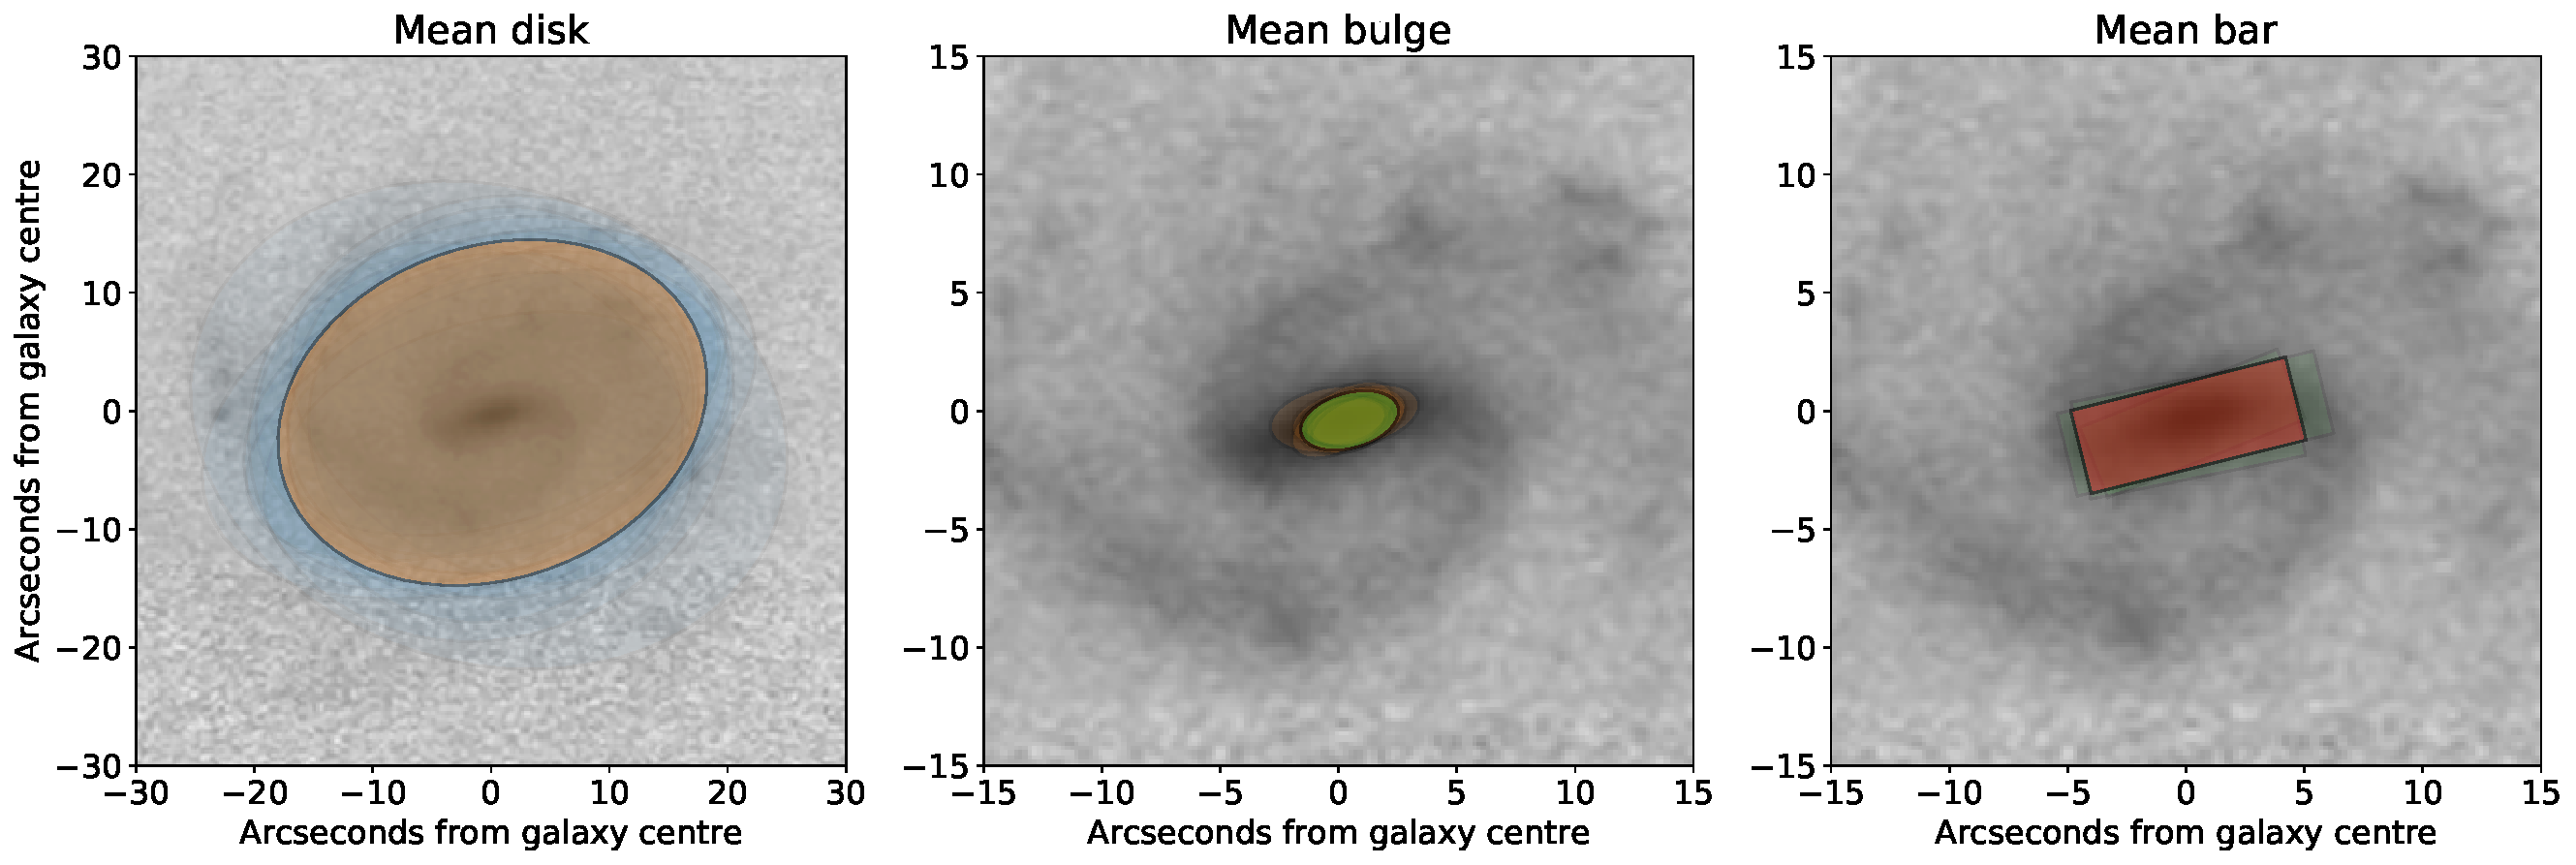
\includegraphics[width=15cm]{images__results/mean_shapes.pdf}
  \caption{Calculated mean components for UGC 4721. The mean disk is shown in orange in the first panel, the mean bulge in green in the second panel and the mean bar in red in the third panel.}
  \label{fig:mean_shapes}
\end{figure*}


\begin{figure}
  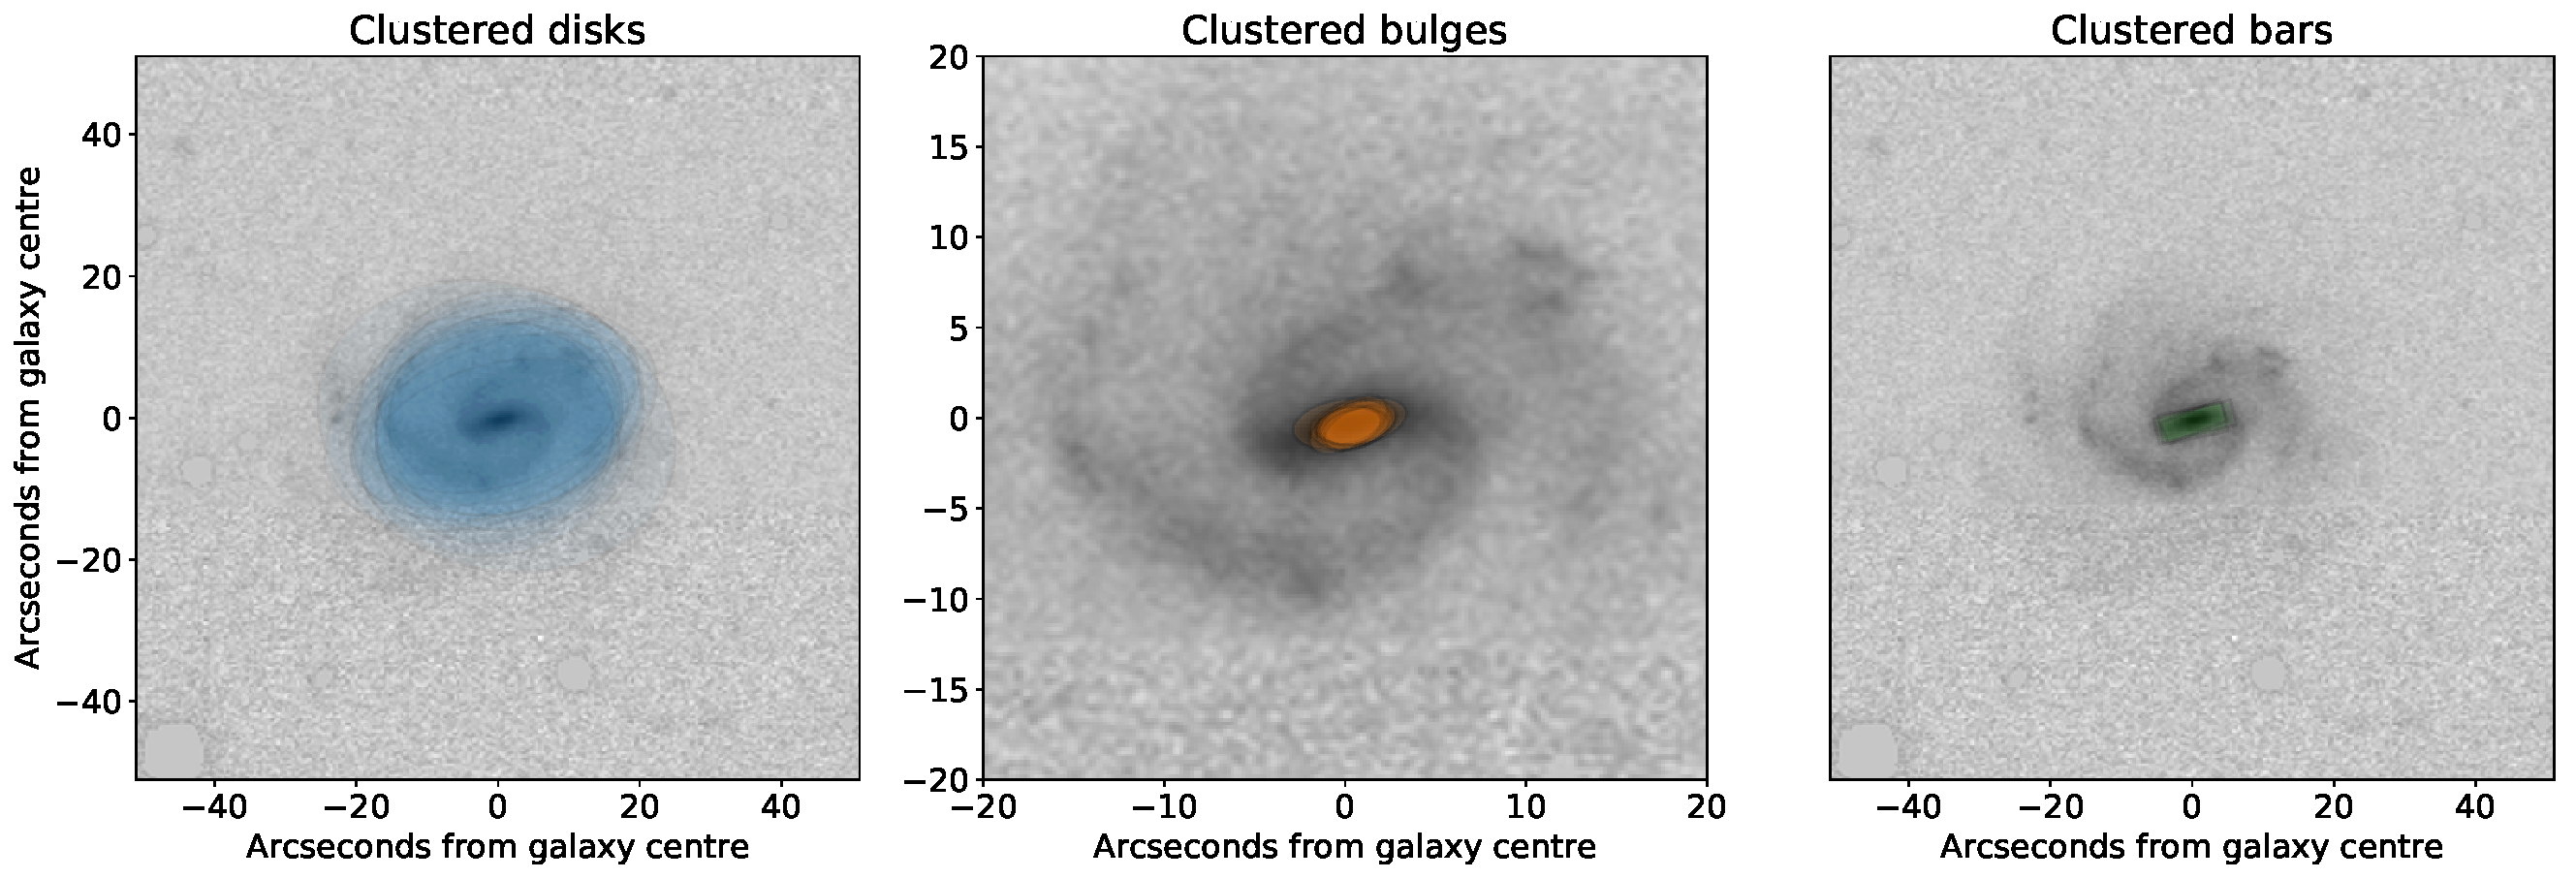
\includegraphics[width=8cm]{images__results/clustered_shapes.pdf}
  \caption{Resulting bulge + disk + bar model for UGC 4721. The disk is shown in blue, the bulge in orange and the bar in green.}
  \label{fig:clustered_shapes}
\end{figure}


\subsubsection{Spiral Arm Aggregation}
\begin{figure}
  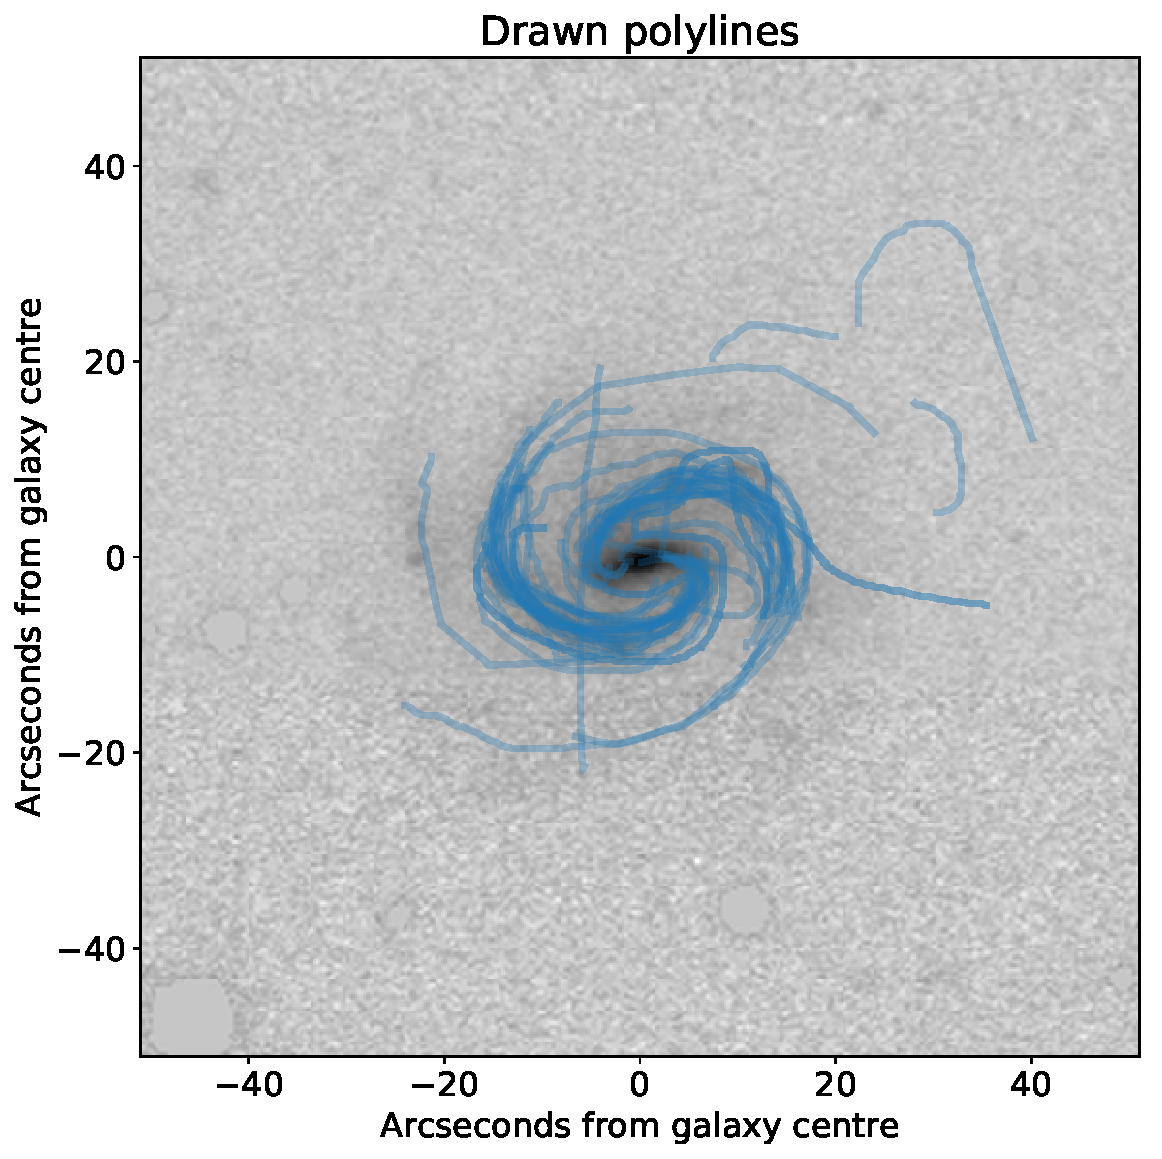
\includegraphics[width=8cm]{images__results/drawn_polylines.pdf}
  \caption{Example of drawn poly-lines for UGC 4721}
  \label{fig:drawn_polylines}
\end{figure}

To cluster drawn spiral arms, we define a custom separation measure to represent how far away one poly-line line is from another. This measure was chosen to be the mean of the squared distances from each vertex in a poly-line to the nearest point (vertex or edge) of another poly-line, added to the mean of the squared distances from the second poly-line to the first. A mathematical description of this measure can be found in Appendix \ref{appendix:clusteringMaths}.

We now make use of this separation measure inside the DBSCAN algorithm to cluster these drawn lines, after removing any self-intersecting drawn arms (as this was deemed an easy method to filter out ``bad'' classifications). The results of this clustering for our example galaxy can be seen in Fig.\ref{fig:arm_clusters}.

\begin{figure}
  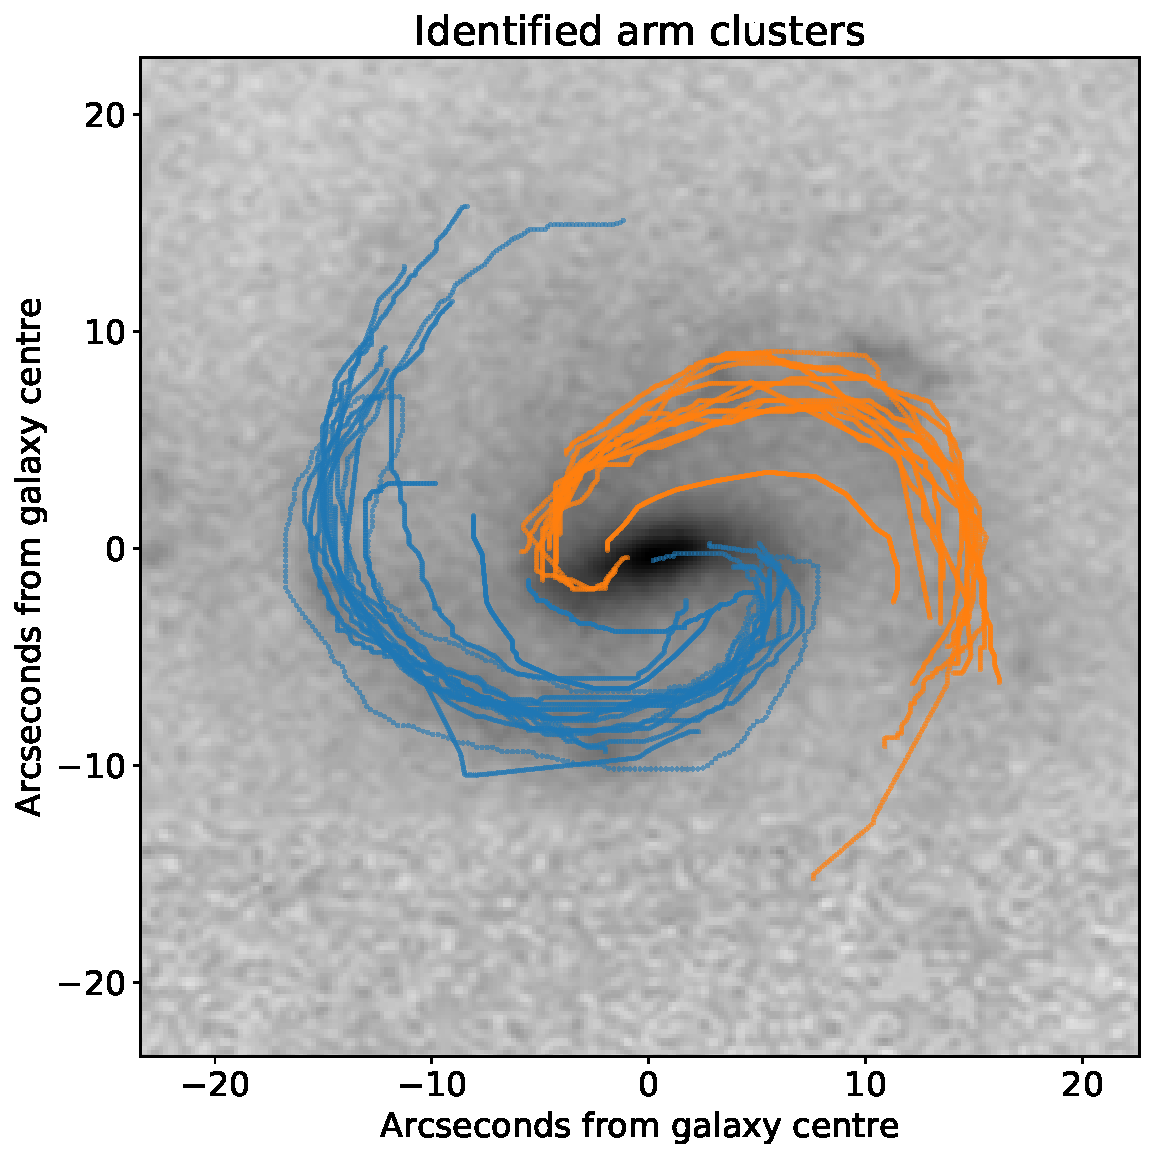
\includegraphics[width=8cm]{images__results/arm_clusters.pdf}
  \caption{The result of clustering drawn poly-lines for UGC 4721 using our separation measure and the DBSCAN clustering algorithm.}
  \label{fig:arm_clusters}
\end{figure}

This clustering method sometimes picks up a small cluster of lines which are a subset of another arm. This is a feature of the separation measure used and is a necessity at this step due to the presence of classifications encompassing both arms with one line.

Once spiral classifications on a galaxy have been clustered into the physical arms they represent, the points are deprojected using the result of a 2D, single-component S\'ersic fit in r-band, provided in the NASA Sloan-atlas value-added catalogue. Once deprojected, points within each drawn poly-line are converted to polar coordinates and unwound using \texttt{numpy.unwrap} to allow model fitting. These unwound points are then cleaned using the Local-outlier-factor algorithm (LOF, \citealt{local-outlier-factor}). For each arm in the cluster, the LOF algorithm was trained on all points not in that arm, and then used to predict whether each point in the arm should be considered an outlier. In this way we clean our data while respecting its grouped nature.

For each arm cluster in each galaxy, a logarithmic spiral model was fitted using Bayesian Ridge Regression, performed using the Scikit-learn python package. Hyperpriors on the noise parameter were chosen by fitting a truncated gamma distribution \comment{citation needed} to the spiral width slider values returned by volunteers (ignoring sliders left at the default or moved to the extremes of allowed values). The logarithmic spiral fit for our example galaxy is shown in Fig.\ref{fig:log_spirals}.

\begin{figure}
  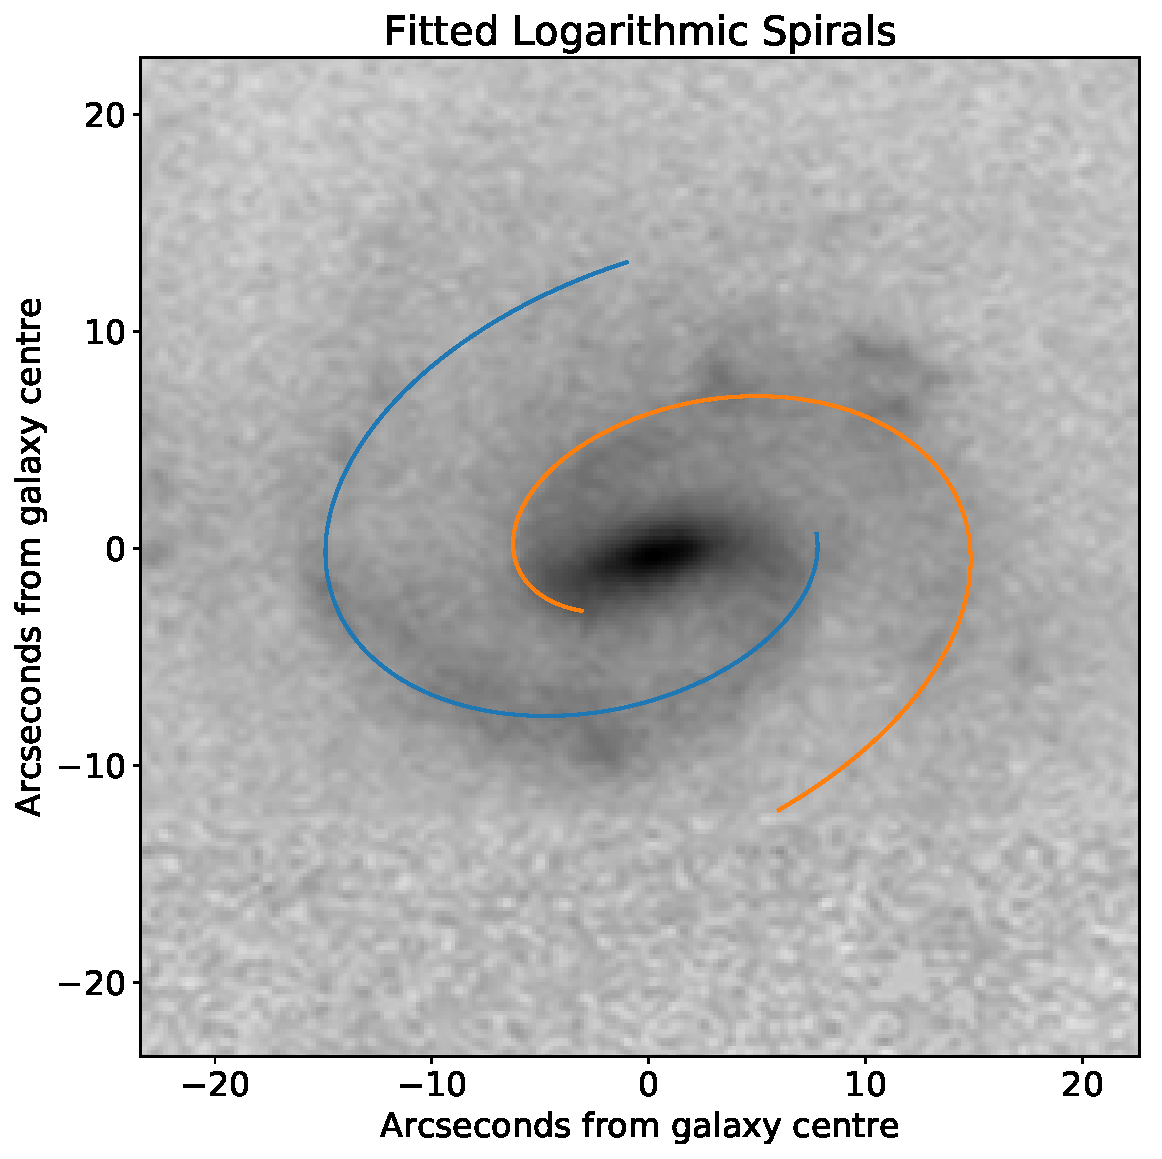
\includegraphics[width=8cm]{images__results/log_spirals.pdf}
  \caption{The fitted logarithmic spirals for UGC 4721}
  \label{fig:log_spirals}
\end{figure}

\end{document}
